\section[Berechenbarkeit]{Berechenbarkeit}



In diesem Kapitel wollen wir zeigen, 
dass es Sprachen gibt, die von keiner \ac{TM} akzeptiert werden können, und
dass es Funktionen gibt, die von keiner \ac{TM} berechnet werden können.


\subsection{Das Gesetz von Church-Turing (Churchsche These)} % 2.6
\begin{These*}[name={[Intuitiv berechenbare Funktionen sind mit \acs*{TM} berechenbar]}]
	Jede intuitiv berechenbare Funktion ist mit einer \ac{TM} (in formalem Sinn) berechenbar.
	
	{\color{gray}
	"`Intuitiv berechenbar"' $\equiv$ man kann einen Algorithmus hinschreiben
	\begin{itemize}
		\item endliche Beschreibung
		\item jeder Schritt effektiv durchführbar
		\item klare Vorschrift
	\end{itemize}
	Status wie Naturgesetz -- nicht beweisbar
	\begin{itemize}[label=\->]
		\item allgemein anerkannt
		\item Weitere Versuche um Berechenbarkeit zu formulieren haben sich als äquivalent zu einer \ac{TM} erwiesen.
	\qedhere
	\end{itemize}
	}
\end{These*}

\begin{Def}\label{def:berechenbar}
 Eine (partielle) Funktion $f:\Sigma^*\rightarrow\Sigma^*$ heißt \emph{berechenbar}, wenn es eine Turingmaschine $\M$ gibt,
 sodass $f$ die von $\M$ berechnete Funktion ist.
\end{Def}
\begin{Bemerkung}
 In der Literatur wird in \autoref{def:berechenbar} oft auch nicht der Begriff \emph{berechenbar}, sondern die Begriffe \emph{Turing-berechenbar} oder \emph{rekursiv} verwendet.
 Die Intention dahinter ist, den Begriff \emph{berechenbar} für "`intuitiv berechenbar"' aufzusparen.
 Wir wollen uns hier aber ganz auf die Churchsche These verlassen und zur Vereinfachung den Begriff auch formal besetzen.
\end{Bemerkung}




\subsection{Nicht berechenbare Funktionen}
\datenote{19.01.2018}

Wir werden nun zeigen, dass es Funktionen gibt, die nicht berechenbar sind.
Unser Vorgehen wird dabei das folgende sein.
\begin{itemize}
 \item Wir zeigen, dass es so viele Turingmaschinen wie natürliche Zahlen gibt.
 \item Wir zeigen, dass es mehr Funktionen als natürliche Zahlen gibt.
\end{itemize}

Da es unendlich viele natürliche Zahlen, Turingmaschinen und Funktionen gibt,
sind die aus der Schule bekannten Formalismen zum Vergleichen von Mengen
(die Größe einer Menge ist die Anzahl ihrer Elemente)
nicht anwendbar.
Wir werden daher über die Existenz von bijektiven Abbildungen argumentieren.

\begin{Bemerkung}
 Zum Verständnis dieses Kapitels ist es nötig, sich mit den Begriffen \emph{injektiv}, \emph{surjektiv} und \emph{bijektiv} vertraut zu machen,
 z.B.\ mit Hilfe von Aufgabe~4 von Übungsblatt~11.
\end{Bemerkung}

Wir führen zunächst die folgenden drei Begriffe ein.
\begin{Def}[Abzählbar, Überabzählbar]
Eine Menge $X$ heißt
\begin{itemize}
 \item \emph{abzählbar unendlich}, wenn es eine bijektive Abbildung zwischen $X$ und $\N$ gibt,
 \item \emph{abzählbar}, wenn $X$ entweder endlich oder abzählbar unendlich ist und
 \item \emph{überabzählbar}, wenn $X$ unendlich ist und es keine bijektive Abbildung zwischen $X$ und $\N$ gibt.
 \qedhere
\end{itemize}
\end{Def}

Ein klassisches Vorgehen, um die Existenz nicht berechenbarer Funktionen zu zeigen, besteht aus den folgenden Schritten.
% In der Literatur wir die  manchmal in einem allgemeineren Kontext gezeigt.
% Wir möchten dieses etwas aufwändigere Vorgehen hier noch kurz erwähnen um mit den entsprechenden (in dieser Vorlesung aber nicht relevanten) Begriffen vertraut zu werden.

% Nach dem Einführen dieser Begriffe werden die folgenden drei Dinge gezeigt.
\begin{enumerate}
 \item Die Menge der Turingmaschinen ist abzählbar.
 \item Die Menge aller Funktionen ist überabzählbar.
 \item Es kann daher nicht zu jeder Funktion auch eine Turingmaschine geben.
\end{enumerate}

Wir wollen hier das folgende, leicht andere, Vorgehen wählen.
Dieses ist weniger allgemein, erlaubt aber etwas leichter nachzuvollziehende Beweise.

\begin{enumerate}
 \item Es gibt für jede Turingmaschine eine natürliche Zahl.
 \item Es gibt für jedes Element der Potenzmenge der natürlichen Zahlen $\calP(\N)$ eine Funktion.
 \item Die Potenzmenge $\calP(\N)$ hat "`sehr viel mehr"' Elemente als $\N$.
 Es kann daher nicht zu jeder Funktion auch eine Turingmaschine geben.
\end{enumerate}





Zur Vereinfachung werden wir uns in diesem Unterkapitel auf das Alphabet $\Sigma=\{0,1\}$ beschränken.

\newcommand{\tmach}{\textit{TMACH}}
\newcommand{\bintonat}{\operatorname{bin}}
\newcommand{\stdnum}{\operatorname{stdnum}}
\newcommand{\nattotm}{\operatorname{nat2tm}}
\newcommand{\bintotm}{\operatorname{bin2tm}}
\newcommand{\langtopower}{\operatorname{lang2power}}
\newcommand{\functopower}{\operatorname{func2power}}

\textbf{Erinnerung: } Die Funktion $\bintonat:\Sigma^*\rightarrow\N$ 
ist die in \autoref{sec:regpl} eingeführte Decodierung von Binärstrings (Wörtern über $\{0,1\}$) in natürliche Zahlen.

Wir möchten zunächst eine bijektive Abbildung zwischen Binärstrings und natürlichen Zahlen definieren.
Die Funktion $\bintonat$ ist hierfür ungeeignet, da führende Nullen ignoriert werden und z.B.\ sowohl $1$ als auch $01$ auf die $1$ abgebildet werden.

Wir führen deshalb die \emph{Standardnummerierung} ein, die auf den folgenden Ideen basiert.
\begin{itemize}
 \item Nummeriere alle Binärstrings der Länge nach; bei gleicher Länge gibt die Funktion $\bintonat$ die Reihenfolge vor.
 \item Es gibt $2^n$ Binärstrings der Länge $n$.
 \item Für einen Binärstring der Länge $n$ gibt es also $\sum\limits_{i=0}^{n-1} 2^i = 2^n-1$ Binärstrings mit kürzerer Länge.
\end{itemize}


\begin{lemma}\label{satz:stdnum}
Die Standardnummerierung $\stdnum: \Sigma^*\rightarrow\N$ 
 $$ \stdnum(a_1\dots a_n)=\begin{cases}
0 & \text{falls } a_1\dots a_n=\Eps\\
2^{n}-1+\bintonat(a_1\dots a_n) & \text{sonst}
\end{cases}$$
ist eine bijektive Abbildung.
\end{lemma}


 \begin{figure}[H]\centering
    \begin{tabular}{rr@{\qquad}l}
    $w\in\{0,1\}^*$ & $\stdnum(w)$ & Berechnung\\ \hline
    $\Eps$ & 0 \\
    0 & 1 & $2^0 + 0$\\
    1 & 2 & $2^0 + 1$\\
    00 & 3 & $2^0 + 2^1 + 0$\\
    01 & 4 & $2^0 + 2^1 + 1$\\
    110 & 13 & $2^0 + 2^1 + 2^2 + 6$\\
    $\godel{\M_r}$ & 72057594037927935 & $2^{55} - 1 + 32977455905055295$
    \end{tabular}

	\caption{Standardnummerierung für einige Beispielwerte; dabei ist $\godel{\M_r}$
	die in \autoref{bsp:CodeVonMr} bestimmte Codierung der 1-Schritt-Rechtsmaschine.}
\end{figure}


\begin{Def}
 Sei $w\in\{0,1\}^*$.
 Die \emph{durch $w$ codierte \ac{TM}} $\M_w$ ist wie folgt definiert.
 $$\M_w=\begin{cases}
\M & \text{falls } w \text{ Code einer \ac{TM} ist und } \godel{\M}=w\\
\D_\mblank & \text{sonst}
\end{cases}$$
Dabei ist $\D_\mblank$ die in \autoref{bsp:simpletms} definierte Druckmaschine.%
\footnote{Für den weiteren Verlauf ist es nicht wichtig, dass wir hier die Druckmaschine gewählt haben. Jede andere \ac{TM} wäre ebenso gut geeignet gewesen.}
\end{Def}

\textbf{Notation:}
Wir verwenden im Folgenden $\tmach$ für die Menge aller Turingmaschinen, bei denen 
\begin{itemize}
 \item jeder Zustand $Q$ von der Transitionsfunktion mindestens einmal auf eine nichtleere Menge abgebildet wird und
 \item jedes Zeichen aus $\Gamma\setminus(\Sigma\cup\{\mblank\})$ von der Transitionsfunktion mindestens einmal auf eine nichtleere Menge abgebildet wird.
\end{itemize}


\begin{Bemerkung}
 Im Folgenden genügt es, wenn wir uns auf \ac{TM}s aus $\tmach$ einschränken.
 Gibt es eine \ac{TM}, die eine Funktion $f$ berechnet, so gibt es auch eine \ac{TM} aus $\tmach$, die $f$ berechnet.
\end{Bemerkung}


\begin{lemma}\label{satz:bintotm}
 Die Abbildung $\bintotm: \Sigma^*\rightarrow \tmach$ 
 $$ \bintotm(w)=\M_w$$
ist surjektiv.
\end{lemma}

\begin{lemma}\label{satz:functopower}
Die Abbildung $\functopower:(\Sigma^*\rightarrow\Sigma^*)\rightarrow \calP(\N)$
$$\functopower(f)=\{\stdnum(w)\mid f(w)=1\}$$
ist surjektiv.
\end{lemma}

 \begin{figure}[H]\centering
    \begin{tabular}{ccc}
    $f$ & $\{w\mid f(w)=1\}$ & $\functopower(f)$\\ \hline
    Inkrement von Binärzahlen & $\{\varepsilon, 0\}$ & $\{0,1\}$\\
    Identitätsfunktion & $\{1\}$ & $\{2\}$\\
    "`alles auf eins"' & $\Sigma^*$ & $\N$
    \end{tabular}

	\caption{$\functopower$ für einige Beispielwerte}
\end{figure}


\begin{Satz}[Cantor]\label{satz:Cantor}
Es gibt keine surjektive Abbildung einer Menge in ihre Potenzmenge.
% Sei $X$ eine beliebige Menge. Es gibt keine surjektive Abbildung 
\end{Satz}
Den Beweis dieses Satzes werden wir später diskutieren.

\begin{Satz}\label{satz:nichtBerechenbar}
 Es gibt Funktionen, die nicht berechenbar sind.
\end{Satz}
\begin{proof}
 Angenommen, jede Funktion $f:\Sigma^*\rightarrow\Sigma^*$ sei berechenbar.
 Dann gibt es für jede Funktion $f$ eine \ac{TM} $\M$ mit $f_\M=f$ und somit eine surjektive Abbildung $g:\tmach\rightarrow(\Sigma^*\rightarrow\Sigma^*)$.
 Nach \autoref{satz:bintotm} und \autoref{satz:functopower} wäre dann aber auch die Abbildung $\functopower\circ g \circ\bintotm\circ \stdnum^{-1}:\N\rightarrow\calP(\N)$ surjektiv.
 Dies steht im Widerspruch zu \autoref{satz:Cantor}.
\end{proof}

Ein zentraler und nicht offensichtlicher Teil dieses Beweises war \autoref{satz:Cantor}.
Wir wollen diesen im restlichen Unterkapitel diskutieren.
Zunächst geben wir einen formalen Beweis.

\begin{proof}[Von \autoref{satz:Cantor}]
Sei $X$ eine beliebige Menge.
Angenommen, es gäbe eine surjektive Abbildung $f:X\rightarrow\calP(X)$.
Betrachte die Menge $Z=\{x\in X\mid x\notin f(x)\}\in\calP(X)$.
Da $f$ surjektiv ist, gibt es ein $z\in X$, sodass $f(z)=Z$.
Nach Definition der Menge $Z$ gilt nun aber $z\in f(z)\Leftrightarrow z\notin f(z)$. Widerspruch!
\end{proof}

Ein Beweis dieser Form wird auch \emph{Diagonalargument} genannt und ist nicht einfach zu verstehen.
Wir werden nun den Beweis für den Spezialfall, dass $X$ eine abzählbare Menge ist, illustrieren.

Da $X$ abzählbar ist, können wir dessen Elemente als unendliche Sequenz $x_0,x_1,\ldots$ aufschreiben.
Wir nehmen nun an, es gäbe eine surjektive Abbildung $f:X\rightarrow\calP(X)$.
Dann können wir $f$ mit Hilfe der folgenden Matrix darstellen.
Zeile $i$ beschreibt dabei das Bild $f(x_i)$. 
Wir haben eine Spalte für jedes $x_j\in X$.
Gilt $x_j\in f(x_i)$, so steht in Eintrag $(i,j)$ ein Y. Ansonsten steht dort ein N.

Da $f$ surjektiv ist, muss es auch für die im formalen Beweis oben erwähnte Menge $Z=\{x\in X\mid x\notin f(x)\}\in\calP(X)$ eine Zeile geben.
Diese Zeile -- wir nehmen an, es sei die Zeile für $f(x_k)$ -- enthält nun in Spalte $j$ immer genau das Inverse des Diagonaleintrags $(j, j)$.
Da der Diagonaleintrag $(k,k)$ nicht invers zu sich selbst sein kann, haben wir einen Widerspruch zu unserer Annahme.


 \begin{figure}[H]\centering

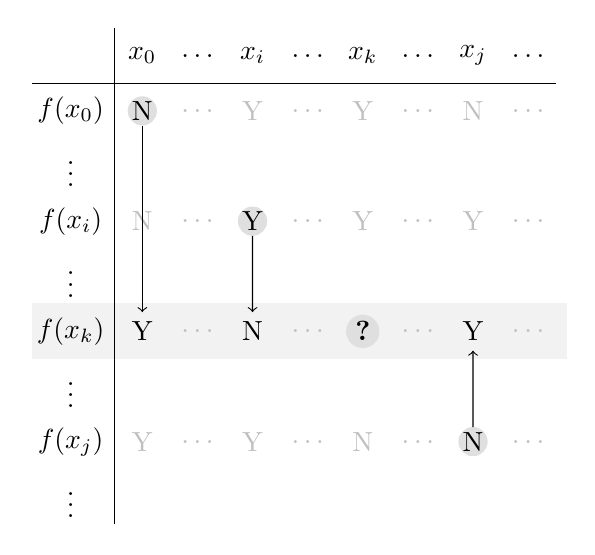
\begin{tikzpicture}[scale=0.7]

\draw[fill=lightgray!20, draw=lightgray!20] (-2,-3.5) rectangle (7.7,-4.5);

\node at (0,1) {$x_0$};
\node at (1,1) {$\dots$};
\node at (2,1) {$x_i$};
\node at (3,1) {$\dots$};
\node at (4,1) {$x_k$};
\node at (5,1) {$\dots$};
\node at (6,1) {$x_j$};
\node at (7,1) {$\dots$};

\node at (-1.3,0) {$f(x_0)$};
\node at (-1.3,-1) {$\vdots$};
\node at (-1.3,-2) {$f(x_i)$};
\node at (-1.3,-3) {$\vdots$};
\node at (-1.3,-4) {$f(x_k)$};
\node at (-1.3,-5) {$\vdots$};
\node at (-1.3,-6) {$f(x_j)$};
\node at (-1.3,-7) {$\vdots$};

\draw (-2, 0.5) to (7.5,0.5);
\draw (-0.5, 1.5) to (-0.5,-7.5);

\node[circle, draw=lightgray!50, fill=lightgray!50, inner sep=0] (00) at (0,0) {N};
\node[lightgray] at (1,0) {$\ldots$};
\node[lightgray] at (2,0) {Y};
\node[lightgray] at (3,0) {$\ldots$};
\node[lightgray] at (4,0) {Y};
\node[lightgray] at (5,0) {$\ldots$};
\node[lightgray] at (6,0) {N};
\node[lightgray] at (7,0) {$\ldots$};

\node[lightgray] at (0,-2) {N};
\node[lightgray] at (1,-2) {$\ldots$};
\node[circle, draw=lightgray!50, fill=lightgray!50, inner sep=0] (ii) at (2,-2) {Y};
\node[lightgray] at (3,-2) {$\ldots$};
\node[lightgray] at (4,-2) {Y};
\node[lightgray] at (5,-2) {$\ldots$};
\node[lightgray] at (6,-2) {Y};
\node[lightgray] at (7,-2) {$\ldots$};

\node (k0) at (0,-4) {Y};
\node[lightgray] at (1,-4) {$\ldots$};
\node (ki) at (2,-4) {N};
\node[lightgray] at (3,-4) {$\ldots$};
\node[circle, draw=lightgray!50, fill=lightgray!50, inner sep=1] (kk) at (4,-4) {\textbf{?}};
\node[lightgray] at (5,-4) {$\ldots$};
\node (kj) at (6,-4) {Y};
\node[lightgray] at (7,-4) {$\ldots$};

\node[lightgray] at (0,-6) {Y};
\node[lightgray] at (1,-6) {$\ldots$};
\node[lightgray] at (2,-6) {Y};
\node[lightgray] at (3,-6) {$\ldots$};
\node[lightgray] at (4,-6) {N};
\node[lightgray] at (5,-6) {$\ldots$};
\node[circle, draw=lightgray!50, fill=lightgray!50, inner sep=0] (jj) at (6,-6) {N};
\node[lightgray] at (7,-6) {$\ldots$};

\draw[->] (00) to (k0);
\draw[->] (ii) to (ki);
\draw[->] (jj) to (kj);

\end{tikzpicture}
	\caption{Illustration des Diagonalarguments beim Beweis des Satzes von Cantor}
\end{figure}


Zum Ende des Unterkapitels möchten wir Diagonalargumente nochmal aus einem anderen Blickwinkel, mit Hilfe eines Rätsels, betrachten.

\textbf{Rätsel:}
Der legendäre \emph{Barbier von Waldkirch} rasierte genau die Männer, die sich nicht selbst rasierten.
Gab es den Barbier von Waldkirch wirklich?

Wir betrachten zum Lösen dieses Rätsels die folgende quadratische Matrix, die je eine Zeile und eine Spalte für jeden Mann aus Waldkirch hat.
Eintrag $(i,j)$ enthält genau dann ein Y, wenn der $i$-te Mann den $j$-ten Mann rasiert.
Gab es den Barbier von Waldkirch, so muss er in einer Zeile zu finden sein.
Nehmen wir an, das sei die $k$-te Zeile.
In dieser Zeile enthält nun der Eintrag in der $i$-ten Spalte immer genau das Inverse des Diagonaleintrags $(i,i)$.
Da der Diagonaleintrag $(k,k)$ nicht invers zu sich selbst sein kann, kann es keine Zeile für den Barbier von Waldkirch geben.

 \begin{figure}[H]\centering

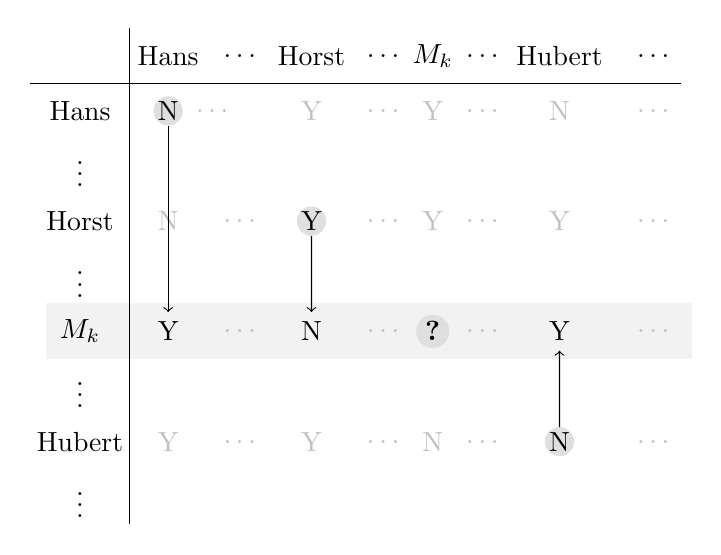
\begin{tikzpicture}[scale=0.7]

\draw[fill=lightgray!20, draw=lightgray!20] (-2,-3.5) rectangle (9.7,-4.5);

\node at (0.2,1) {Hans};
\node at (1.5,1) {$\dots$};
\node at (2.8,1) {Horst};
\node at (4.1,1) {$\dots$};
\node at (5,1) {$M_k$};
\node at (5.9,1) {$\dots$};
\node at (7.3,1) {Hubert};
\node at (9,1) {$\dots$};

\node at (-1.4,0) {Hans};
\node at (-1.4,-1) {$\vdots$};
\node at (-1.4,-2) {Horst};
\node at (-1.4,-3) {$\vdots$};
\node at (-1.4,-4) {$M_k$};
\node at (-1.4,-5) {$\vdots$};
\node at (-1.4,-6) {Hubert};
\node at (-1.4,-7) {$\vdots$};

\draw (-2.3, 0.5) to (9.5,0.5);
\draw (-0.5, 1.5) to (-0.5,-7.5);

\node[circle, draw=lightgray!50, fill=lightgray!50, inner sep=0] (00) at (0.2,0) {N};
\node[lightgray] at (1,0) {$\ldots$};
\node[lightgray] at (2.8,0) {Y};
\node[lightgray] at (4.1,0) {$\ldots$};
\node[lightgray] at (5,0) {Y};
\node[lightgray] at (5.9,0) {$\ldots$};
\node[lightgray] at (7.3,0) {N};
\node[lightgray] at (9,0) {$\ldots$};

\node[lightgray] at (0.2,-2) {N};
\node[lightgray] at (1.5,-2) {$\ldots$};
\node[circle, draw=lightgray!50, fill=lightgray!50, inner sep=0] (ii) at (2.8,-2) {Y};
\node[lightgray] at (4.1,-2) {$\ldots$};
\node[lightgray] at (5,-2) {Y};
\node[lightgray] at (5.9,-2) {$\ldots$};
\node[lightgray] at (7.3,-2) {Y};
\node[lightgray] at (9,-2) {$\ldots$};

\node (k0) at (0.2,-4) {Y};
\node[lightgray] at (1.5,-4) {$\ldots$};
\node (ki) at (2.8,-4) {N};
\node[lightgray] at (4.1,-4) {$\ldots$};
\node[circle, draw=lightgray!50, fill=lightgray!50, inner sep=1] (kk) at (5,-4) {\textbf{?}};
\node[lightgray] at (5.9,-4) {$\ldots$};
\node (kj) at (7.3,-4) {Y};
\node[lightgray] at (9,-4) {$\ldots$};

\node[lightgray] at (0.2,-6) {Y};
\node[lightgray] at (1.5,-6) {$\ldots$};
\node[lightgray] at (2.8,-6) {Y};
\node[lightgray] at (4.1,-6) {$\ldots$};
\node[lightgray] at (5,-6) {N};
\node[lightgray] at (5.9,-6) {$\ldots$};
\node[circle, draw=lightgray!50, fill=lightgray!50, inner sep=0] (jj) at (7.3,-6) {N};
\node[lightgray] at (9,-6) {$\ldots$};

\draw[->] (00) to (k0);
\draw[->] (ii) to (ki);
\draw[->] (jj) to (kj);

\end{tikzpicture}
	\caption{Illustration des Diagonalarguments beim Rätsel des Barbiers von Waldkirch}
\end{figure}




\subsection{Sprachakzeptanz und Berechenbarkeit}
Wir möchten nun die Idee von Berechenbarkeit auch auf die zweite Aufgabe von Turingmaschinen, das Akzeptieren von Sprachen, übertragen.
Wir definieren dafür die Menge der Sprachen, für die eine Lösung für das Wortproblem (also $w\in L$?) berechnet werden kann, wie folgt.

\begin{Def}[name={[Entscheidbarkeit]}]
	Sei $\M$ eine \ac{TM}.
	Wir sagen $\M$ \emph{entscheidet} $L\subseteq\Sigma^*$, falls die folgenden beiden Eigenschaften gelten:
	\begin{enumerate}
	\item $\M$ akzeptiert $L$.
	\item $\M$ hält für jede Eingabe an.
	\end{enumerate}
	
    Eine Sprache $L\subseteq\Sigma^*$ heißt \emph{entscheidbar}, falls es eine \ac{TM} gibt, die $L$ entscheidet.\footnote{
    Ein alternativer in der Literatur auch oft verwendeter Begriff für "`entscheidbar"' ist "`rekursiv"'.}
\end{Def}


\begin{Satz}\label{satz:NichtEntscheidbareSprache}
 Es gibt Sprachen, die nicht entscheidbar sind.
\end{Satz}

\draftnote{24.01.2018}
\begin{proof}
Wähle $\Sigma=\{0,1\}$ 
und definiere die Funktion \mbox{$\langtopower:\Sigma^*\rightarrow \calP(\N)$}
$$\langtopower(L)=\{\stdnum(w) \mid w\in L\}$$
(analog zu \autoref{satz:functopower}) und zeige, dass diese surjektiv ist.
Führe anschließend analog zum Beweis von \autoref{satz:nichtBerechenbar} einen Widerspruchsbeweis.
Annahme: Jede Sprache $L\subseteq\Sigma^*$ sei entscheidbar. Also gibt es eine surjektive Abbildung $g:\tmach\rightarrow\Sigma^*$.
Somit wäre auch 
$$\langtopower\circ g \circ\bintotm\circ \stdnum^{-1}:\N\rightarrow\calP(\N)$$
surjektiv.
Dies steht im Widerspruch zu \autoref{satz:Cantor}.
\end{proof}

 \begin{figure}[H]\centering

\begin{tikzpicture}[
countable/.style={ellipse,draw, minimum height=2cm, minimum width=12mm, node distance = 21mm},
uncountable/.style={ellipse,draw, minimum height=3cm, minimum width=12mm, node distance = 21mm},
]
 \node (nat) [countable] at (0,0) {};
 \node (lnat) [yshift=2mm] at (nat.north) {$\N$};
 \node (strings) [countable, right=of nat] {};
 \node (lstrings) [yshift=2mm] at (strings.north) {$\{0,1\}^*$};
 \node (tms) [countable, right=of strings] {};
 \node (ltms) [yshift=2mm] at (tms.north) {$\tmach$};
 \node (langs) [uncountable, right=of tms] {};
 \node (llangs) [yshift=2mm] at (langs.north) {$\calP(\Sigma^*)$};
 \node (powernat) [uncountable, right=of langs] {};
 \node (lpowernat) [yshift=2mm] at (powernat.north) {$\calP(\N)$};
 
 \node (e1nat) [yshift=-6mm] at (nat.north) {$\bullet 23$};
 \node (e2nat) [yshift=-16mm] at (nat.north) {$\bullet 42$};
 
 \node (e1strings) [yshift=-8mm] at (strings.north) {$\bullet 110$};
 \node (e2strings) [yshift=-14mm] at (strings.north) {$\bullet 00$};

 \node (e1tms) [yshift=-6mm] at (tms.north) {$\bullet \M_R$};
 \node (e2tms) [yshift=-16mm] at (tms.north) {$\bullet \D_\mblank$};
 
 \node (e1langs) [yshift=-12mm] at (langs.north) {$\bullet \{110\}$};
 \node (e2langs) [yshift=-20mm] at (langs.north) {$\bullet L(0^*)$};
 
 \node (e1powernat) [yshift=-15mm] at (powernat.north) {$\bullet \{5,7\}$};
 \node (e2powernat) [yshift=-8mm] at (powernat.north) {$\bullet \N$};


 
 \draw[->, bend left] (nat) to node[auto] {$\stdnum^{-1}$} (strings);
 \draw[->, bend left] (strings) to node[auto] {$\bintotm$} (tms);
 \draw[->, bend left] (tms) to node[auto] {$g$} (langs);
 \draw[->, bend left] (langs) to node[auto] {$\langtopower$} (powernat);
 \draw[->, bend right, dashed] (nat) to node[below] {$\langtopower\circ g \circ\bintotm\circ \stdnum^{-1}$} (powernat);
\end{tikzpicture}

	\caption{Konkatenierte Abbildung aus dem Widerspruchsbeweis zu \autoref{satz:NichtEntscheidbareSprache}}
\end{figure}


\begin{Def}[Charakteristische Funktion]
Sei $L\subseteq\Sigma^*$ eine Sprache. Die \emph{charakteristische Funktion} $\chi_L:\Sigma^*\rightarrow\{0,1\}$ ist wie folgt definiert:
\begin{equation*}
\chi_L(w)=\begin{cases}
1 & \text{falls } w\in L\\
0 & \text{falls } w\notin L           
\end{cases}
\qedhere
\end{equation*}
\end{Def}

Der folgende Satz zeigt uns nun einen direkten Zusammenhang zwischen den beiden Aufgaben einer Turingmaschine, 
dem Berechnen von Funktionen und dem Akzeptieren von Wörtern.
\begin{Satz}\label{satz:characFunc}
    Sei $\{0,1\}\subseteq\Sigma$.
    Eine Sprache $L\subseteq\Sigma^*$ ist genau dann entscheidbar, wenn die charakteristische Funktion $\chi_L$
    berechenbar ist.
\end{Satz}




\hide{
\subsection{Typ-0 und Typ-1 Sprachen}
%\ptnote{checkpoint}
% \begin{Def}[name={[NTM]}]
% 	\acf{NTM} ist ein Tupel $(Q,\Sigma,\Gamma,\delta,q_0,\blank,F)$, wobei alles wie bei einer \ac{DTM} außer $\delta: Q\x\Gamma\-> \wp(Q\x\Gamma\x\{N,L,R\})$.\\
% 	Konfiguration und Berechnungsrelation wie gehabt.
% \end{Def}

\begin{Def}[name={[Akzeptanz, Entscheidbarkeit, Semi-Entscheidbarkeit]}]
	Sei $M$ \ac{TM}.
	\begin{itemize}
	\item $M$  \emph{akzeptiert} $w\in\Sigma^*$, falls $q_0w
          \vdash^* uq'v$ Haltekonfiguration und $q'\in F$
	\item $M$ \emph{akzeptiert} $L\subseteq\Sigma^*$, falls $M$ akzeptiert $w \<-> w\in L$
	\item $M$ \emph{entscheidet} $L\subseteq\Sigma^*$, falls $M$ akzeptiert $L$ und $M$ hält für jede Eingabe an.
	\item $L\subseteq\Sigma^*$ ist \emph{semi-entscheidbar} (rekursiv aufzählbar), falls $\exists M$, die $L$ akzeptiert.
	\item $L\subseteq\Sigma^*$ ist \emph{entscheidbar} (rekursiv), falls $\exists M$, die $L$ entscheidet.
	\end{itemize}
\end{Def}
\begin{Def}[name={[Laufzeit und Platzbedarf einer \acs*{TM}]}]
	Laufzeit und Platzbedarf einer \ac{TM} $M:$
	
	Laufzeit : $T_M(w) =
	\begin{cases}
		\parbox{.74\textwidth}{\raggedleft Anzahl der Schritte einer kürzesten Berechnung, die zur Akz. von $w$ führt (falls $\exists$)}\\[-1em]
		\text{1, sonst}
	\end{cases}
	$\\
	Platzbedarf : $S_M(w) =
	\begin{cases}
		\parbox{.7\textwidth}{\raggedleft geringster Platzbedarf (Länge einer Konf.) einer akz. Berechnung von $w$ (falls $\exists$)}\\[-1em]
		\text{1, sonst}
	\end{cases}
	$
\textbf{Zeitbeschränkt mit $t(n)$}: $\forall w\in\Sigma^*: |w|\leq n \=> T_M(w)\leq t(n)$,\\
platzbeschränkt analog.
\end{Def}
\begin{Satz}[name={[Zu jeder \acs*{NTM} gibt es \acs*{DTM}]}]\label{satz:6.1}
	Zu jeder \ac{NTM} gibt es eine \ac{DTM} $M'$, sodass
	\begin{itemize}
	\item $M'$ akzeptiert $L(M)$
	\item $M'$ terminiert gdw. $M$ terminiert
	\item Falls $M$ zeit- und platzbeschränkt ist mit $t(n)$
          bzw. $s(n)$ ($n=$ Länge der Eingabe), dann ist $M'$
          zeitbeschränkt mit $2^{O(t(n))}$ und platzbeschränkt mit
          $O(s(n)\cdot t(n))$. 
	\end{itemize}
\end{Satz}\vspace{-2em}
\begin{proof}
	Die Konfigurationen von $M$ bilden einen Baum, dessen Kanten durch $\vdash$ gegeben sind. Er ist endlich verzweigt, hat aber ggf. unendlich lange Äste.
	
	Definiere eine (Mehrband-)\ac{DTM}, die den Konfigurationsbaum
        systematisch durchläuft und akzeptiert, sobald eine
        Haltekonfiguration erreicht ist, in der $M$ akzeptiert. 
	
	Die \ac{DTM} terminiert ebenfalls, wenn alle Blätter des Baumes besucht worden sind, ohne dass eine akzeptierende Konfiguration gefunden wurde.
	
	Baumsuche mit Kontrollinformation und bereits besuchten Konf. auf ein Extraband.
	\begin{itemize}
	\item Tiefensuche? Nicht geeignet, sie könnte in unendlichen Ast laufen.
	\item Breitensuche? OK, aber Platzbedarf $O(2^{t(n)}\cdot s(n))$
	\item iterative deepending\,: Tiefensuche mit vorgegebener Schranke, bei erfolgloser Suche Neustart mit erhöhter Schranke. \qedhere
	\end{itemize}
\end{proof}
Nächstes Ziel: Charakterisierung von Typ-1 Sprachen.
\begin{Def}[name={[$\DTAPE$ und $\NTAPE$]}]\
\begin{itemize}
\item $\DTAPE(s(n)):$ Menge der Sprachen, die von einer \ac{DTM} in Platz $s(n)$ akzeptiert werden können.
\item $\NTAPE(s(n)):$ Wie für $\DTAPE$, aber mit \ac{NTM}. \qedhere
\end{itemize}
\end{Def}
\begin{Bemerkung}\
	\newcommand{\underarrowset}[2]{%
		\underset{%
			\mathclap{%
				\overset{\displaystyle\uparrow}{\mathclap{#1}}%
			}%
		}{#2}%
	}
	\begin{enumerate}
	\item Für "`$s(n)\leq n$"' betrachte 2-Band \ac{TM}, bei denen die Eingabe read-only ist und nur das zweite Arbeitsband der Platzschranke unterliegt (so ist $s(n)$ sublinear möglich).
	\item Jede Platzbeschränkung impliziert Laufzeitschranke.\\
	Angenommen Platzschranke $s(n)$\\
	$\curvearrowright$ \ac{TM} hat nur endlich viele Konfigurationen
	\[ N := \underarrowset{%
			\parbox{\widthof{\scriptsize Eingabeband}}{\raggedright\scriptsize Kopfpos. im Eingabeband}\hspace{1cm}
		}{n\vphantom{|}}
		|Q| \quad\cdot\quad
		\underarrowset{\parbox{2.2cm}{\scriptsize\centering mögliche Inhalte des Arbeitsbands}}{|\Gamma|}^{s(n)}
		\ \cdot\
		\underarrowset{\hspace{1.7cm}\parbox{2cm}{\scriptsize Kopfpos. auf\\ Arbeitsband}}{s(n)}
		\in 2^{O(\log n + s(n))}
	\]
	\item \ac{DTM} mit Platzschranke\,: $M$ entscheidet,\\
	falls sie akzeptiert, dann in weniger als $N$ Schritten,\\
	falls nach $N$ Schritten keine Terminierung erfolgt\\
	\quad$\curvearrowright$ Endlosschleife -- Abbruch
	\item \ac{NTM}\,: nutze den \ac{ND} optimistisch aus\,:\\
	falls eine akzeptierende Berechnung existiert, dann muss es eine Berechnung ohne wiederholte Konfiguration geben.
	\end{enumerate}
\end{Bemerkung}
\begin{Satz}[name={[$L\in\DTAPE(n),\ L\in\NTAPE(n)$]}]\label{satz:6.2}\
	\begin{itemize}
	\item $L\in\DTAPE(n) \curvearrowright\ \exists$ \ac{DTM}, die $L$ in Zeit $2^{O(n)}$ entscheidet.
	\item $L\in\NTAPE(n)$ analog.
	\end{itemize}
\end{Satz}\vspace{-2em}
\begin{proof}
	siehe oben.
\end{proof}
\begin{Bemerkung}
	Die Klasse $\NTAPE (n)$ heißt auch \ac{LBA}.
\end{Bemerkung}
%
\begin{Satz}\label{satz:6.3}
	$\mathcal L_1=\mathrm{NTAPE}(n)$
\end{Satz}
\begin{proof}\
\begin{itemize}
	\item["`\=>"'\,:] Sei $G=(N,\Sigma,P,S)$ Typ-1 Grammatik für $L$.\\
		Konstruiere \ac{NTM} $M$ mit $L=L(M),\ \Gamma = \Sigma\cup N\cup\{\blank\}$
		\begin{enumerate}
		\item $M$ rät nicht deterministisch eine Position auf
                  dem Band und eine Produktion $\alpha\-> \beta$. Falls $\beta$ gefunden wird, ersetze durch $\alpha$, weiter bei 1.
		\item Falls Bandinhalt $=S$ \quad stop, akzeptiert.
		\end{enumerate}
		Dieses Verfahren terminiert.
	\item["`\<="'\,:] %
	Gegeben: \ac{NTM} $M$ linear beschränkt.\\
	Gesucht: Typ-1 Grammatik $\mathcal{G}$ mit $L(\mathcal{G})=L(M)$\\
	Idee: 
	\begin{align*}
		a_1\cdots a_n &\-->
			\pmqty{a_1\\a_1} \pmqty{a_2\\a_2} \pmqty{(q,a)\\a_3} \pmqty{a_4\\a_4} \pmqty{a_n\\a_n}
			&&\begin{matrix}\text{Spur 1}\\\text{Spur 2}\end{matrix}\\
	\shortintertext{ad\footnotemark\ Spur 1: Alphabet $\Gamma\cup(Q\x\Gamma) = \triangle$}
		P' &\begin{cases}
			(q,a) &\-> (q',a')   \quad q\in Q,a\in\Gamma\\
			(q,a)b &\-> a'(q',b) \quad b\in\Gamma\\
			b(q,a) &\-> (q',b)a'
		\end{cases}
		& &\begin{aligned}
			\delta(q,a) &\ni (q',a',N)\\
			\delta(q,a) &\ni (q',a',R)\\
			\delta(q,a) &\ni (q',a',L)
		\end{aligned}
	\end{align*}\footnotetext{ad $\approx$ zur}%
	Def. $\widetilde{uqav} = u(q,a)v\ ,\ u,v\in\Gamma^*,a\in\Gamma$\\
	Es gilt: $uqav\vdash^* k' \curvearrowleftright \widetilde{uqav} \overset{*}{\=>} \widetilde{k'}$ mit Produktion $P'$.
	
	Def. $\mathcal{G}$ durch $N = \{S\}\dotcup\triangle\x\Sigma$
	\begin{align*}
		\text{mit } P &= \\
		S &\-> \pmqty{(q_0,a)\\a} &&\forall a\in\Sigma\\
		S &\-> S\pmqty{a\\a} &&\forall a\in\Sigma\\
		\pmqty{\alpha\\a}
			&\-> \pmqty{\beta\\a}
			&&\begin{aligned}
				\forall \alpha\->\beta &\in P'\\
				\alpha,\beta &\in\triangle
			\end{aligned}\\
		\pmqty{\alpha_1\\a_1}\pmqty{\alpha_2\\a_2}
			&\-> \pmqty{\beta_1\\a_1}\pmqty{\beta_2\\a_2}
			&&\begin{aligned}
				\forall \alpha_1\alpha_2\->\beta_1\beta_2 &\in P'\\
				\alpha_i,\beta_i &\in\triangle
			\end{aligned}\\
		\pmqty{x\\a} &\-> a
			&&\begin{aligned}
				x&\in\Gamma\\
				a&\in\Sigma
			\end{aligned}\\
		\pmqty{(q',x)\\a} &\-> a
			&&\begin{aligned}
				x&\in\Gamma, q'\in F, \delta (q',x)=\emptyset\\
				a&\in\Sigma
			\end{aligned}
	\end{align*}
	\begin{align*}
		S &\xRightarrow{*} \pmqty{(q_0,a_1)\\a_1}\pmqty{a_2\\a_2}\dots\pmqty{a_n\\a_n}\\
		&\phantom{{}\xRightarrow{*}{}}\ \acs*{TM}\ \,\dots\\
		&\xRightarrow{*} \pmqty{x_1\\a_1}\dots\pmqty{(q',x_i)\\a_i}\dots\pmqty{x_n\\a_n}\\
		&\xRightarrow{*} a_1\dots a_i\dots a_n
	\end{align*}
	Damit gesehen $L(\mathcal{G})\subseteq L(M)$\\
	Rückrichtung: selbst \qedhere
	\end{itemize}
\end{proof}

\begin{Satz}
	Die Typ-1 Sprachen sind abgeschlossen unter {\thinmuskip=6mu$\cup,\cap,\cdot,{}^*$} und Komplement.
\end{Satz}
\begin{proof}
	Zu $\cup$ und $\cap$ betrachte \ac{NTM}.\\
	Für $\cdot$ und $^*$ konstruiere Grammatik.\\
	ad Komplement "`2. \acsu{LBA}-Problem\footnote{\acs*{LBA} = \acl*{LBA} -- 1964 Kuroda}"' bis 1987, dann gelöst durch Immerman und Szelepcsényi.
\end{proof}
\begin{Bemerkung}
  1. \ac{LBA}-Problem (1964): Ist $\mathrm{NTAPE}(n) = \mathrm{DTAPE}(n)$? Bisher ungelöst.
\end{Bemerkung}
\begin{Satz}
	Das Wortproblem für Typ-1 Sprachen ist entscheidbar.
\end{Satz}
\begin{proof}
	\begin{align*}
		L\in\mathcal{L}_1 &\curvearrowleftright L\in\mathrm{NTAPE}(n)\\
		&\curvearrowright \text{nach \autoref{satz:6.2}: $L$ entscheidbar}
	\end{align*}
	Nach \autoref{satz:6.1} sogar mit \ac{DTM}.
\end{proof}
Die Rückrichtung "`L entscheidbar. $\xcancel{\curvearrowright}\ L$ ist Typ-1 Sprache"' gilt nicht!

\begin{Satz}\label{satz:6.6}
	$\mathcal{L}_0 = \ac{NTM}$
\end{Satz}
\begin{proof}
	\begin{itemize}
	\item["'\=>"'] Konstruktion einer \ac{NTM} $M$ wie in \autoref{satz:6.3}, aber ohne Platzbeschränkung.
	\item["'\<="'] Konstruktion analog zu \autoref{satz:6.3} + Startsymbol $S'$
	\begin{align*}
		S' &\-> \pmqty{\blank\\\Eps} S' \pmqty{\blank\\\Eps} &&\text{Schaffe Platz für Berechnung von }M\\
		S' &\-> S\\
	\shortintertext{Erweitere $N$}
		&= \{S',S\}\cup\triangle\x(\Sigma\cup\{\Eps\})\\
	\shortintertext{Neue Löschregeln:}
		\pmqty{x\\ \Eps } &\-> \Eps &&\forall x\in\Gamma\\
		\rotatebox{90}{$\Rsh$}\ &\mathrlap{\text{die einzigen
                                          Regeln, die Typ-1 Bedingung verletzen.}} \tag*{\qedhere}
	\end{align*}
	\end{itemize}
\end{proof}

\begin{Satz}[name={[Abgeschlossenheit von Typ-0 Sprachen]}]\label{satz:Typ-0-abgeschl}
	Die Typ-0 Sprachen sind unter $\thinmuskip=6mu\cup,\cap,\cdot,{}^*$ abgeschlossen.
\end{Satz}
\begin{proof}
	Konstruiere \ac{NTM} für $\thinmuskip=6mu\cup,\cap$ ; Typ-0-Grammatiken für $\cdot$ und $^*$.
\end{proof}

\begin{Bem}
	Typ-0 Sprachen sind \emph{nicht} unter Komplement abgeschlossen!
\end{Bem}
}


\subsection{Das Halteproblem}
Aus den bisherigen Sätzen wissen wir nur, 
dass es nicht berechenbare Funktionen und unentscheidbare Sprachen geben muss.
Es besteht also noch Hoffnung, dass kein praxisrelevantes Problem betroffen ist.
In diesem Kapitel werden wir nun aber für ein ganz konkretes praxisrelevantes Problem die Unentscheidbarkeit nachweisen.

% Schreibe ab jetzt $M_w$ für die Maschine mit Gödelnummer $w$. Falls
% $w$ kein gültiger Code für eine \ac{TM}, dann sei $M_w$ eine beliebige fest
% \ac{TM} $M$ mit $L(M) = \varnothing$.

\begin{Def}[name={[Spezielles Halteproblem]}]
  Das spezielle Halteproblem besteht aus allen Codes von \ac{TM}s, die
  anhalten, falls sie auf den eigenen Code angesetzt werden.
  \begin{align*}
    K &= \{ w \in \{0,1\}^* \mid M_w \text{ angesetzt auf }w\text{
        hält} \}\qedhere
  \end{align*}
\end{Def}
\begin{Satz}\label{satz:speziellesHalteproblem}
  Das spezielle Halteproblem ist unentscheidbar.
\end{Satz}

Wir geben zunächst einen kurzen formalen Beweis mit Hilfe eines Diagonalarguments
und diskutieren diesen anschließend.
\begin{proof}
  Angenommen, $\M_\text{€}$ wäre eine \ac{TM}, die $K$ entscheidet.
  Dann gibt es auch eine \ac{TM} $\M_\textsf{evil}$, (siehe \autoref{fig:Mevil})
  die zunächst $\M_\text{€}$ auf ihre Eingabe anwendet.\footnote{
  Der Name $\M_\text{€}$ soll den hohen Wert dieser \ac{TM} betonen.
  Gäbe es einen Algorithmus zur Terminierungsanalyse, könnten wir damit viele Probleme in der Softwareentwicklung lösen.
  Der Name $\M_\textsf{evil}$ soll suggerieren, dass diese \ac{TM} unsere entsprechenden Hoffnungen zunichte macht.
  }
  Falls $\M_\text{€}$ akzeptiert, dann geht $\M_\textsf{evil}$ in eine Endlosschleife. 
  Falls $\M_\text{€}$ nicht akzeptiert, dann hält $\M_\textsf{evil}$ an. Nun gilt:
  \begin{eqnarray*}
  \M_\text{€} \text{ akzeptiert } \godel{\M_\textsf{evil}} 
  &\stackrel{\text{Def.\ von } K}{\text{gdw.}} & \M_\textsf{evil} \text{ angesetzt auf } \godel{\M_\textsf{evil}} \text{ hält }\\
  &\stackrel{\text{Def.\ von } \M_\textsf{evil}}{\text{gdw.}} & \M_\text{€} \text{ akzeptiert } \godel{\M_\textsf{evil}} \text{ nicht}
  \end{eqnarray*}
  Ein Widerspruch.
\end{proof}

 \begin{figure}[H]\centering
  \begin{tikzpicture}
   \node (0) at (0,0) {$\M_{\chi_K}$};
   \node (init) at (-1.1,.2) {};
   \node (1) at (2,0) {$\D_\mblank$};
   \draw[->] (init) to (0);
   \draw[->] (0) to node[auto] {$1$} (1);
   \draw[->,loop right] (1) to node {$\Gamma$} (1);
  \end{tikzpicture}
  \caption{Definition der \ac{TM} $\M_\textsf{evil}$ aus dem Beweis von \autoref{satz:speziellesHalteproblem} mit Hilfe eines Flussdiagramms.
  Die \ac{TM} $\M_{\chi_K}$ verhält sich wie $\M_\text{€}$, aber statt zu akzeptieren (bzw. nicht zu akzeptieren), schreibt diese 1 (bzw. 0) auf das Band und hält (siehe \autoref{satz:characFunc}).}
  \label{fig:Mevil}
 \end{figure}



% Dieser Beweis verwendete wieder ein Diagonalargument, wir werden den Beweis nun graphisch illustrieren.

Wir wollen diesen Beweis nun wieder graphisch illustrieren.
Die folgende Matrix enthält eine Spalte für jedes Wort $w\in\{0,1\}^*$.
Wir wählen z.B. $w_i=\stdnum^{-1}$ und aus der Bijektivität von $\stdnum$ folgt, dass jedes $w\in\{0,1\}^*$ einmal vorkommt.
Wir haben außerdem unendlich viele Zeilen.
In Zeile $i$ steht die durch $w_i$ codierte \ac{TM}.
Aus \autoref{satz:bintotm} folgt also, dass jede \ac{TM} in mindestens einer Zeile vorkommt.
In Eintrag $(i,j)$ steht ein Y, wenn $\M_{w_i}$ angesetzt auf $w_j$ hält, und ansonsten ein N. %, wenn $\M_{w_i}$ angesetzt auf $w_j$ nicht hält
(Wir können diese Tabelleneinträge zwar nicht berechnen, doch dies ist hier nicht wichtig.)
Die \ac{TM} $\M_\text{€}$, deren Existenz wir im Beweis angenommen haben (die für alle $w\in\{0,1\}^*$ entscheidet, ob $\M_w$ angesetzt auf $w$ hält) ist eine \ac{TM}, die alle Diagonaleinträge in unserer Matrix bestimmen kann.
Die daraufhin konstruierte \ac{TM} $\M_\textsf{evil}$ (siehe \autoref{fig:Mevil}) muss in irgendeiner Zeile vorkommen.
Sei $w_k$ das Wort, das die \ac{TM} $\M_\textsf{evil}$ codiert (also $\M_{w_k} = \M_\textsf{evil}$).
Die Definition von $\M_\textsf{evil}$ sagt uns, dass die Zeile $\M_{w_k}$ in Spalte $i$ immer genau das Gegenteil (Y/N) des Diagonaleintrags $(i,i)$ enthält. Die Betrachtung des Diagonaleintrags $(k,k)$ zeigt uns den Widerspruch.
Die Annahme der Existenz von $\M_\text{€}$ war also falsch. 

 \begin{figure}[H]\centering

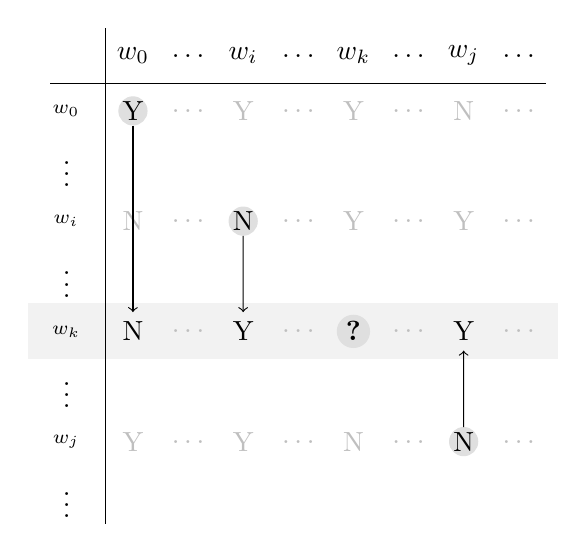
\begin{tikzpicture}[scale=0.7]

\draw[fill=lightgray!20, draw=lightgray!20] (-1.9,-3.5) rectangle (7.7,-4.5);

\node at (0,1) {$w_0$};
\node at (1,1) {$\dots$};
\node at (2,1) {$w_i$};
\node at (3,1) {$\dots$};
\node at (4,1) {$w_k$};
\node at (5,1) {$\dots$};
\node at (6,1) {$w_j$};
\node at (7,1) {$\dots$};

\node at (-1.2,0) {$\M_{w_0}$};
\node at (-1.2,-1) {$\vdots$};
\node at (-1.2,-2) {$\M_{w_i}$};
\node at (-1.2,-3) {$\vdots$};
\node at (-1.2,-4) {$\M_{w_k}$};
\node at (-1.2,-5) {$\vdots$};
\node at (-1.2,-6) {$\M_{w_j}$};
\node at (-1.2,-7) {$\vdots$};

\draw (-1.5, 0.5) to (7.5,0.5);
\draw (-0.5, 1.5) to (-0.5,-7.5);

\node[circle, draw=lightgray!50, fill=lightgray!50, inner sep=0] (00) at (0,0) {Y};
\node[lightgray] at (1,0) {$\ldots$};
\node[lightgray] at (2,0) {Y};
\node[lightgray] at (3,0) {$\ldots$};
\node[lightgray] at (4,0) {Y};
\node[lightgray] at (5,0) {$\ldots$};
\node[lightgray] at (6,0) {N};
\node[lightgray] at (7,0) {$\ldots$};

\node[lightgray] at (0,-2) {N};
\node[lightgray] at (1,-2) {$\ldots$};
\node[circle, draw=lightgray!50, fill=lightgray!50, inner sep=0] (ii) at (2,-2) {N};
\node[lightgray] at (3,-2) {$\ldots$};
\node[lightgray] at (4,-2) {Y};
\node[lightgray] at (5,-2) {$\ldots$};
\node[lightgray] at (6,-2) {Y};
\node[lightgray] at (7,-2) {$\ldots$};

\node (k0) at (0,-4) {N};
\node[lightgray] at (1,-4) {$\ldots$};
\node (ki) at (2,-4) {Y};
\node[lightgray] at (3,-4) {$\ldots$};
\node[circle, draw=lightgray!50, fill=lightgray!50, inner sep=1] (kk) at (4,-4) {\textbf{?}};
\node[lightgray] at (5,-4) {$\ldots$};
\node (kj) at (6,-4) {Y};
\node[lightgray] at (7,-4) {$\ldots$};

\node[lightgray] at (0,-6) {Y};
\node[lightgray] at (1,-6) {$\ldots$};
\node[lightgray] at (2,-6) {Y};
\node[lightgray] at (3,-6) {$\ldots$};
\node[lightgray] at (4,-6) {N};
\node[lightgray] at (5,-6) {$\ldots$};
\node[circle, draw=lightgray!50, fill=lightgray!50, inner sep=0] (jj) at (6,-6) {N};
\node[lightgray] at (7,-6) {$\ldots$};

\draw[->] (00) to (k0);
\draw[->] (ii) to (ki);
\draw[->] (jj) to (kj);

\end{tikzpicture}
	\caption{Illustration des Diagonalarguments beim Beweis der Unentscheidbarkeit des speziellen Halteproblems}
\end{figure}

\begin{Korollar}\label{kor:6.11}
    Das Komplement von $K$
  $$\overline{K} = \{w \in\{0,1\}^* \mid M_w\text{ angesetzt auf }w\text{
        hält nicht} \}$$
  ist nicht entscheidbar.
\end{Korollar}
\begin{proof}
	Angenommen, $\overline{K}$ sei entscheidbar durch eine \ac{TM} $\M$.
	Betrachte \ac{TM} $\M'$, die zunächst $\M$ ausführt und dann das Ergebnis negiert.
	$\M'$ entscheidet $K$.
	Widerspruch zu \autoref{satz:speziellesHalteproblem}.
\end{proof}




\begin{Def}[name={[Semi-Entscheidbarkeit]}]
	Eine Sprache $L\subseteq\Sigma^*$ heißt \emph{semi-entscheidbar}, falls es eine \ac{TM} gibt, die $L$ akzeptiert.\footnote{
	Ein alternativer in der Literatur auch oft verwendeter Begriff für "`semi-entscheidbar"' ist "`rekursiv aufzählbar"'.}
\end{Def}


\begin{lemma}[name={[$K$ ist semi-entscheidbar]}]\label{lemma:Ksemi-entscheidbar}
	$K$ ist semi-entscheidbar.
\end{lemma}
\begin{proof}
  Die wie folgt konstruierte \ac{TM} $\M$ akzeptiert $K$.
  Sei $w$ die Eingabe. 
  Führe die universelle \ac{TM} für $M_w$ mit Eingabe $w$ aus.
  Falls diese Simulation stoppt, geht $\M$ in einen akzeptierenden Zustand und hält.
\end{proof}
% \begin{Def}[name={[length-lexicographic order]}]
% 	Die \emph{length-lexicographic order} auf $\{0, 1\}^*$ (mit $0<1$) ist definiert durch
% 	\begin{align*}
% 		v \leq w \<=> &\ |v| < |w|\\
% 		\vee &\ v = w\\
% 		\vee &\ |v| = |w| \text{ und } \exists u\in \{0, 1\}^*\\
% 		& \text{mit } v = u0v' \text{ und } w = u1w'
% 	\end{align*}
% \end{Def}
% \begin{Satz}[name={[$\leq:$ totale Ordnung]}]\
% 	\begin{itemize}
% 		\item $\leq$ ist totale Ordnung auf $\{0, 1\}^*$
% 		\item $\exists$ bijektive Abbildung $w: \N \to \{0, 1\}^*$ mit $i \leq j \to w(i) \leq w(j)$
% 	\end{itemize}
% \end{Satz}
% \begin{Def}[name={[Diagonalsprache]}]
% 	Sei $M_i$ die Turingmaschine mit Gödelnummer $\ulcorner M_i\urcorner = w(i)$.
% 	(falls $w(i)$ kein gültiger Code, dann sei $M_i$ eine beliebige \ac{TM} mit $L(M_i) = \varnothing$). Die \emph{Diagonalsprache}
% 	\[D = \{w(i) \mid w(i) \notin L(M_i)\}\]
% 	das heißt $M_i$ akzeptiert $w(i)$ nicht.
% \end{Def}
% \begin{Satz}[name={[$D$ ist nicht entscheidbar]}]\label{satz:speziellesHalteproblem}
% 	$D$ ist nicht entscheidbar.
% \end{Satz}
% \begin{proof}
% 	Angenommen, $\exists M$, die $D$ entscheidet.\\
% 	$M$ muss in Aufzählung vorkommen, das heißt $\exists j\in \N$, sodass $M = M_j$.
% 	Wende $M_j$ auf $w(j)$ an:
% 	\begin{itemize}
% 		\item $M_j$ stoppt/ja: $w(j) \in L(M_j) = D \qquad \lightning$ Def. von $D$
% 		\item $M_j$ stoppt/nein: $w(j) \notin L(M_j) = D \quad \lightning$ Def. von $D$ \qedhere
% 	\end{itemize}
% \end{proof}
% \begin{Korollar}\label{kor:6.11}
% 	$\overline{D} = \{w(i) \mid M_i\text{ akzepztiert }w(i) \}$ ist nicht entscheidbar.
% \end{Korollar}
% \begin{proof}
% 	Angenommen, $\overline{D}$ sei entscheidbar durch $M$. Dann entscheidet $M'\ D$. $M'$ führt
% 	zuerst $M$ aus und negiert das Ergebnis. $\lightning$ \autoref{satz:speziellesHalteproblem}
% \end{proof}
% \begin{lemma}[name={[$\overline{D}$ ist semi-entscheidbar]}]
% 	$\overline{D}$ ist semi-entscheidbar.
% \end{lemma}
% \begin{proof}
% 	Bei Eingabe $w$
% 	\begin{itemize}
% 		\item Falls $w$ kein gültiger Code: stop mit Ergebnis nein.
% 		\item Falls $w$ gültiger Code, dann $\exists i$, sodass $ww = \left\ulcorner M_j
% 		\right\urcorner w(i) \qquad w = w(i)$
% 	\end{itemize}
% 	Wende $U$ auf $ww$ an.\\
% 	Insgesamt: \ac{TM}, die $\overline{D}$ akzeptiert.
% \end{proof}



\begin{Satz}[name={[{$L,\overline{L}$ semi-entscheidbar $\=> L$ entscheidbar}]},restate={[name=Wiederholung]repeatSatz613}]\label{satz:6.13}
    Wenn eine Sprache $L$ und ihr Komplement $\overline{L}$ semi-entscheidbar sind, dann ist $L$ entscheidbar.
\end{Satz}
\begin{proof}
	Sei $\M$ eine \ac{TM}, die $L$ akzeptiert, und sei $\overline{\M}$ eine \ac{TM}, die $\overline{L}$ akzeptiert.
	Führe $\M$ und $\overline{\M}$ "`parallel"' mit der gleichen Eingabe aus (z.B. mit einer 2-Band-\ac{TM}).\newline
	Eine \ac{TM} muss anhalten, da für alle Eingaben $w$ entweder $w \in L$ oder $w \in \overline{L}$ gilt.
	\begin{itemize}
	\item Falls $\M$ akzeptiert -- halte und akzeptiere.
	\item Falls $\overline{\M}$ akzeptiert -- halte aber akzeptiere nicht. \qedhere
	\end{itemize}
\end{proof}

\begin{Korollar}\label{kor:6.11}
    Das Komplement des speziellen Halteproblems $\overline{K}$
    ist nicht semi-{\linebreak}entscheidbar.
\end{Korollar}
\begin{proof}
Nach \autoref{lemma:Ksemi-entscheidbar} ist $K$ semi-entscheidbar. 
Angenommen, $\overline{K}$ sei auch semi-entscheidbar.
Dann wäre $K$ nach \autoref{satz:6.13} entscheidbar.
Widerspruch zu \autoref{satz:speziellesHalteproblem}.
\end{proof}


\begin{Def}[Reduktion]\ \\
  Seien $U, V \subseteq \Sigma^*$ Sprachen.
  \emph{$U$ ist auf $V$ reduzierbar (Notation: $U \preceq V$)}, falls eine totale, berechenbare Funktion
  $f:\Sigma^* \to \Sigma^*$ existiert, sodass
  \[
    \forall w \in \Sigma^*:w \in U \iff f(w) \in V. \qedhere
  \]

\end{Def}
\begin{lemma}\label{lemma:reduktion}
  Falls $U \preceq V$ gilt und die Sprache $V$ \mbox{(semi-)entscheidbar} ist, dann ist auch die Sprache $U$
  \mbox{(semi-)entscheidbar}.
\end{lemma}
\begin{proof}
  Sei $\M_V$ eine \ac{TM}, die ein (Semi-)Entscheidungsverfahren für $V$ implementiert,
  und sei $\M_f$ eine \ac{TM}, die $f$ berechnet.
  Konstruiere $\M_U$ wie folgt:
  \begin{itemize}
  \item Wende erst $\M_f$ auf die Eingabe $w$ an.
  \item Führe dann $\M_V$ auf dem Ergebnis $f(w)$ aus.
  \end{itemize}
  Da $f$ total ist, hält $\M_f$ immer.
  $\M_U$ hält also genau dann, wenn $\M_V$ hält.
\end{proof}

\begin{Bemerkung} \autoref{lemma:reduktion} wird oft verwendet, um zu zeigen, dass eine Sprache \emph{nicht} \mbox{(semi-)entscheidbar} ist.
Dafür nutzen wir die Negation der Implikation.
\begin{itemize}
 \item $U \preceq V$ und $U$ unentscheidbar $\Rightarrow$ $V$ unentscheidbar.
 \item $U \preceq V$ und $U$ nicht semi-entscheidbar $\Rightarrow$ $V$ nicht semi-entscheidbar.
 \qedhere
\end{itemize}
\end{Bemerkung}

\begin{Def}[name={[Halteproblem]}]
	Das \emph{Halteproblem} ist definiert durch
	\[H = \{\godel{\M}\# w \mid M \text{ angesetzt auf } w \text{ hält}\}. \qedhere\]
\end{Def}
\begin{Satz}[name={[$H$ ist unentscheidbar]}]\label{satz:H ist unentscheidbar}
	$H$ ist unentscheidbar.
\end{Satz}
\begin{proof}
  Wir zeigen die Reduktion $K \preceq H$ mittels der Funktion $f(w) = w\#w$.
  Die Funktion ist offensichtlich total und berechenbar.
  \begin{align*}
   w \in K & \quad\Longleftrightarrow\quad \text{ $\M_w$ hält bei Eingabe $w$ an}\\
   & \quad\Longleftrightarrow\quad \underbrace{w\#w}_{f(w)} \in H \qedhere
  \end{align*}
\end{proof}
% \begin{proof}
% 	Angenommen, $M_0$ entscheidet $H$.\\
% 	Konstruiere $M'$ wie folgt:\\
% 	Bei Eingabe $w$ bestimme $i$, sodass $w = w(i)$\\
% 	Verwende $M_0$ um festzustellen, ob $\ulcorner M_i\urcorner w$ anhält.\\
% 	Antwort von $M_0:$\\
% 	nein: $\begin{aligned}[t]
% 		&\curvearrowright w(i) \notin L(M_i)\\
% 		&\curvearrowright M'\text{ akzeptiert }w\text{ nicht}.
% 	\end{aligned}$\\
% 	ja: Führe $\ulcorner M_i\urcorner w$ mit $U$ aus (muss ja terminieren) und akzeptiere entsprechend das Ergebnis von $U$.\\
% 	Insgesamt: $M'$ entscheidet $\overline{D} \qquad \lightning$ \autoref{kor:6.11}\\
% 	$\curvearrowright M_0$ existiert nicht.
% \end{proof}
\begin{Satz}[name={[$H$ ist semi-entscheidbar]}]
	$H$ ist semi-entscheidbar.
\end{Satz}
\begin{proof}
  Die wie folgt konstruierte \ac{TM} $\M$ akzeptiert $H$.
  Zunächst simuliert $\M$ die universelle \ac{TM} auf der Eingabe $\godel{M}\#w$.
  Falls diese Simulation stoppt, geht $\M$ in einen akzeptierenden Zustand und hält.
\end{proof}


\begin{Def}[name={[Halteproblem auf leerem Band $H_\Eps$]}]
	Das \emph{Halteproblem auf dem leerem Band} ist definiert durch
	\[H_\Eps = \{\godel{\M}\# w \mid M \text{ angesetzt auf das leere Band hält}\}. \qedhere\]
\end{Def}
\begin{Satz}[name={[$H_\Eps$ ist unentscheidbar]}]
\label{satz:HalteproblemLeeresBand}
	$H_\Eps$ ist unentscheidbar.
\end{Satz}
\begin{proof}
  Wir zeigen die Reduktion $H \preceq H_\Eps$ mittels der
  Funktion $f$, die eine Eingabe $v$ der Form $v = w\#x$ auf eine \ac{TM} $\godel{\M_{w,x}}$ (siehe unten) und ansonsten auf $0$ abbildet.%
  \footnote{Wir hätten hier auch jedes andere Wort statt 0 wählen können, das nicht in $H_\Eps$ liegt.}
  \[ f(v) = \begin{cases} \godel{\M_{w,x}} & \text{falls } v = w\#x \\ 0 & \text{sonst}\end{cases} \]
  Dabei ist $\M_{w,x}$ eine \ac{TM}, die folgendermaßen funktioniert.
  \begin{itemize}
  \item Zuerst schreibt $\M_{w,x}$ das Wort $x$ auf das leere Band und läuft zum Anfang.
  \item Dann wendet $\M_{w,x}$ die durch $w$ codierte \ac{TM} $\M_w$ auf $x$ an.
  \end{itemize}
  Offensichtlich ist $f$ total und berechenbar und es gilt $v\in H$ gdw.\ $f(v) \in H_\Eps$.
\end{proof}
% \begin{proof}
% 	Angenommen, $M_\varepsilon$ entscheidet $H_\Eps$.\\
% 	Konstruiere $M'$ (mit Hilfe von $M_\varepsilon$), sodass $M'$ entscheidet $H$.\\
% 	\begin{tabular}{r@{ }l}
% 	$M':$ & Bei Eingabe $\ulcorner M\urcorner w$.\\
% 	& Konstruiere $M^*$, $M^*$ schreibt zuerst $w$ aufs (leere) Band und 
% 	startet dann $M$ auf $w$.\\
% 	& Wende $M_\varepsilon$ auf $\ulcorner M^*\urcorner$ an.
% 	\end{tabular}\\
% 	$\curvearrowright M'$ entscheidet $H \qquad \lightning$ \autoref{satz:H ist unentscheidbar}
% \end{proof}

 % Latex-Qelle von M. Geffken
Nun betrachten wir \ac{TM}s vom Blickwinkel der von ihnen berechneten
(partiellen) Funktionen. 

\begin{Satz}[Satz von Rice]\ \\
  Sei $R$ die Menge aller (partiellen) \ac{TM}-berechenbaren Funktionen und $S$
  eine nichtleere, echte Teilmenge davon (also $\varnothing \subsetneq S \subsetneq R$).
  Dann ist die Sprache
  $$C_S=\{\godel{\M} \mid \M \text{ berechnet eine Funktion aus }S\}$$
  unentscheidbar.
\end{Satz}
\begin{proof}
  Sei $\varnothing \subsetneq S \subsetneq R$ beliebig.
  Angenommen, es gibt eine \ac{TM} $\M_\text{€}$, die $C_S$ entscheidet.
  Sei $\Omega \in R$ die überall undefinierte Funktion. 
  Wir betrachten zwei Fälle.
  \begin{itemize}
   \item Fall 1: $\Omega \in S$
   
     Da $S\subsetneq R$ gilt, gibt es eine berechenbare Funktion $f \in R \setminus S$.
     Sei $M_f$ eine \ac{TM}, die $f$ berechnet.
     Sei $w\in\{0,1\}^*$ beliebig.
     Wir definieren zunächst die \ac{TM} $\M_{w, f}$ wie folgt:
     $\M_{w, f}$ führt zunächst die durch $w$ codierte \ac{TM} $\M_w$ auf der leeren Eingabe aus.
     Falls $\M_w$ anhält, wendet $\M_{w, f}$ dann $\M_f$ auf die tatsächliche Eingabe an.\\
     ($\M_{w, f}$ sollte also zunächst eine Kopie der Eingabe speichern,
     z.B.\ als 2-Band-\ac{TM}, die ein Band für die Eingabe verwendet.)
     
     Die von $\M_{w, f}$ berechnete Funktion ist also:
     $$f_{\M_{w, f}}=\begin{cases}
                      f & \text{falls } \M_w \text{ auf dem leerem Band hält,}\\
                      \Omega & \text{sonst.}
                      \end{cases}$$
     
     Wir definieren nun die \ac{TM} $\M_\textsf{Evil}$ (abhängig von $w$) wie folgt:
     $\M_\textsf{Evil}$ nimmt die Eingabe $w$, konstruiert die \ac{TM} $\M_{w, f}$ und wendet $\M_\text{€}$ auf $\godel{\M_{w, f}}$ an.
     Nun gilt:
     \begin{align*}
      M_\text{€} \text{ akzeptiert } \godel{\M_{w, f}}
      &\iff \godel{\M_{w, f}} \text{ berechnet eine Funktion in }S\\
      &\iff \godel{\M_{w, f}} \text{ berechnet }\Omega\\ % \text{ ($f_{\M_{w, f}} \in \{\Omega, f\}, \Omega \in S, f \notin S$ )}\\
      &\iff \M_w \text{ hält \emph{nicht} auf dem leeren Band}
    \end{align*}
    Also entscheidet $\M_\textsf{Evil}$ die Sprache $H_\Eps$. Widerspruch zu \autoref{satz:HalteproblemLeeresBand}.
    \item Fall 2: $\Omega \notin S$
    
    Analog zu Fall 1. \qedhere
  \end{itemize}
\end{proof}



\hide{

Bemerkung: Korollar zu 
\begin{Korollar}
	$\mathcal{L}_0 \supsetneqq \mathcal{L}_1$
\end{Korollar}
\begin{proof}
	$K$ ist unentscheidbar (also $\notin \mathcal{L}_1$), aber semi-entscheidbar (also $\in \mathcal{L}_0$).
\end{proof}
\emph{\textbf{Fragen:}}
\begin{enumerate}
	\item Ist $\mathcal{L}_1$ = Menge der entscheidbaren Sprachen?
	\item[--] Nein:\\
	\begin{minipage}[t]{.7\linewidth}
	Konstruiere eine Kodierung von Typ-1 Grammatiken als Worte
        $w\in\{0,1\}^*$. Die Grammatik zum Wort $w$ sei $G_w$; falls
        $w$ kein sinnvoller Kode ist, setze $G_w = (\{S\}, \{0,1\},
        \{\}, S)$ die leere Grammatik.
        
	Die \emph{Diagonalsprache} $D = \{w \in\{\0,1\}^* \mid w\notin
        L(G_w)\}$ ist entscheidbar, weil das Wortproblem für Typ-1  
	Sprachen entscheidbar, aber es $\nexists w$, sodass $L(G_w) =
        D$. Beweis durch Widerspruch.
	\end{minipage}\quad
	\begin{tabular}[t]{M{c} | *4{M{c}@{ }}}
		\ &w_1&w_2&w_3&\cdots\\\hline
		G_1 &\\
		G_2 &\\
		G_3 &\\
		\vdots&
	\end{tabular}
	\item Ist $\mathcal{L}_0$ = Menge aller Sprachen?
	\item[--] Nein: $\overline{K} \notin \mathcal{L}_0$
\end{enumerate}


\subsection{Eigenschaften von entscheidbaren und semi-entscheidbaren Sprachen}
\begin{Satz}[name={[Eigenschaften von Entscheidbarkeit]}]
\label{thm:eigensch-von-entsch}
  Seien $L_1$ und $L_2$ entscheidbar. Dann sind $\overline{L_1}$, $\overline{L_2}$, $L_1 \cup L_2$ und $L_1 \cap L_2$ entscheidbar.
\end{Satz}\vspace{-1.5em}
\begin{proof}
  Übung oder selbst.
\end{proof}
\begin{Satz}[name={[Eigenschaften von Semi-Entscheidbarkeit]}]
  Seien $L_1$ und $L_2$ semi-entscheidbar. Dann sind $L_1 \cup L_2$ und $L_1 \cap L_2$ semi-entscheidbar.
\end{Satz}
\begin{proof}
  vgl. \autoref{satz:Typ-0-abgeschl}.
\end{proof}
\csname repeatSatz613\endcsname*
\begin{Satz}
  Die Menge der semi-entscheidbaren Sprachen ist \emph{nicht}
  unter Komplement abgeschlossen.
\end{Satz}
\begin{proof}
  Laut \autoref{satz:speziellesHalteproblem} und \autoref{kor:6.11} sind das spezielle Halteproblem $K$ und $\overline{K}$ nicht entscheidbar.
  
  $K$ ist semi-entscheidbar, aber nicht $\overline{K}$.
\end{proof}


\subsection{Weitere unentscheidbare Probleme}
\draftnote{1.2.17}
\paragraph[\acf*{PCP}]{\acf{PCP}}\ \\
\emph{Gegeben:}\\
Endliche Folge von Wortpaaren $K=((x_1, y_1), \dots, (x_k, y_k))$ mit $x_i, y_i \in \Sigma^+$

\emph{Gesucht:}\\
Indexfolge $i_1, \dots, i_n \in \{1, \dots, k\}\ (n \geq 1)$, sodass $x_{i_1} \cdots x_{i_n}=y_{i_1} \cdots y_{i_n}$

Die Folge $i_1, \dots, i_n$ (falls diese existiert) heißt \emph{Lösung} des Korrespondenzproblems $K$.
\begin{Bsp*}
\begin{align*}
	K &=((\underbrace{1,101}_{x_1, y_1}), (\underbrace{10, 00}_{x_2, y_2}), (\underbrace{011, 11}_{x_3, y_3}))\\
\shortintertext{besitzt die Lösung $(1,3,2,3)$, denn}
	x_1 x_3 x_2 x_3 &= \underbrace{1 \cdot 01}_{y_1}\underbrace{1 \cdot 1}_{y_3}\underbrace{0 \cdot 0}_{y_2}\underbrace{11}_{y_3} = y_1 y_3 y_2 y_3
\end{align*}
\end{Bsp*}\vspace{-1em}
\emph{Frage:}
\begin{align*}
  x_1&=001 & x_2&=01 & x_3&=01 & x_2&=10\\
  y_1&=0  & y_2&=011 & y_3&=101  & y_2&=001\\
\end{align*}
Besitzt dieses \ac{PCP} eine Lösung? Ja, aber mit $66$ Indizes [Schöning, S.124]
\begin{Bemerkung}\ \\
  Offensichtlich ist das \ac{PCP} semi-entscheidbar: Systematisches
  Ausprobieren von Indexfolgen findet Lösung nach endlicher Zeit,
  \emph{sofern es eine gibt}.
\end{Bemerkung}
Ziel: \ac{PCP} ist unentscheidbar. Vorbereitung:
Es interessiert uns ab hier nur, ob das Problem eine Lösung hat oder nicht.
\paragraph[\acf*{MPCP}]{\acf{MPCP}}\ \\
\emph{Gegeben:} wie bei \ac{PCP}

\emph{Gesucht:} Lösung des \acsu{CP} mit $i_1=1$
\begin{lemma}[name={[MPCP $\preceq$ PCP]}]
    \ac{MPCP} $\preceq$ \ac{PCP}
\end{lemma}
\begin{proof}
	Betrachte \ac{MPCP} $K=((x_1,y_1),\dots(x_k,y_k))$ über $\Sigma$.\\
	Sei $\Sigma'=\Sigma\uplus\{\#,\$\}$ \\
	Für ein Wort $w=a_1\dots a_n\in\Sigma^+$ sei
	\begin{align*}
		\bar w &= \#a_1\#a_2\#\dots\#a_n\#\\
		\grave w &= \#a_1\#a_2\#\dots\#a_n &&\text{(am Ende kein \#)}\\
		\acute w &= \phantom{\#}a_1\#a_2\#\dots\#a_n\# &&(\text{am Anfang kein }\#)
	\end{align*}
	Definiere nun
	\[ f(K) = (\underbrace{(\bar x_1,\grave y_1)}_1, \underbrace{(\acute x_1, \grave y_1)}_2, \underbrace{(\acute x_2,\grave y_2)}_{2+1}, \dots, \underbrace{(\acute x_k,\grave y_k)}_{k+1}, \underbrace{(\$,\#\$)}_{k+2}) \]
	eine totale berechenbare Funktion.
	
	Zeige $K \in \ac{MPCP} \<==> f(K) \in \ac{PCP}$:
	
	"`$\==>$"': $1, i_2, \dots, i_n$ Lösung für $K$\\
	$\curvearrowright\ 1, i_{2}+1, \dots, i_{n}+1, k+2$ Lösung für $f(K)$
	
	"`$\<==$"':
  \begin{enumerate}
  \item \label{it:mpcp-pcp-only-if-1} Sei $i_1, \dots, i_n$ Lösung für $f(K)$, in der das Paar $k+2$ höchstens einmal vorkommt.\\
  $\curvearrowright$  Durch die Stuktur der Worte gilt für Lösungen immer: $ i_1=1,\ i_n=k+2 $ (ansonsten fehlt am Anfang oder am Ende das Symbol $\#$)\\
  Es gilt ferner für $1 < j < n$
  \begin{itemize}
  \item $i_j \neq 1$, da in der $x$-Konkatenation sonst $\#$ doppelt vorkommt, was in der $y$-Konkatenation nicht möglich ist.
  \item $i_j \neq k+2$, da $k+2$ per Annahme nur einmal vorkommt.
  \end{itemize}
  Also gilt für $1 < j < n$: $i_j \in \{2, \dots, k+1\}$.\\
	$\curvearrowright 1, i_{2}-1, \dots, i_{n-1}-1$ Lösung für $K$
\item Sei $i_1, \dots, i_n$ Lösung für $f(K)$, in der das Paar $k+2$ mehrmals vorkommt.
  Dann gibt es auch eine Lösung $i_m,\dots,i_{m+l}$ mit $1 \le m \le m+l \le n$ sodass $k+2$ nur einmal vorkommt (ohne Beweis).
  Weiter bei \ref{it:mpcp-pcp-only-if-1}.
  \end{enumerate}

\end{proof}
Es reicht nun zu zeigen, dass \ac{MPCP} unentscheidbar ist!

\begin{lemma}[name={[H $\preceq$ \ac{MPCP}]}] 
	H $\preceq$ \ac{MPCP}
\end{lemma}
\begin{proof}
	\ac{TM} $M=(Q,\Sigma,\Gamma,\delta,q_0,\blank,F)$ und Eingabewort $w\in\Sigma^*$.
	
	Gesucht: totale berechenbare Funktion, die $(\ulcorner M \urcorner, w) \mapsto \underbrace{(x_1,y_1),\dots,(x_k,y_k)}_k$, sodass\\
	$\ulcorner M \urcorner w\in H \text{ gdw } K$ eine Lösung als \ac{MPCP} besitzt.
	
	Idee: Definiere $K$ so, dass die Berechnung von $M$ simuliert wird.\\
	Alphabet für $K: \triangle = \Gamma\cup Q\cup\{\#\}$\\
	$(x_1,y_1) = (\#,\#q_0w\#)$
	\begin{enumerate}
	\item Kopieren
		\[ (a,a)\quad, a\in\Gamma\cup\{\#\} \]
	\item Transition ($a \in \Gamma$)
		\begin{alignat*}{2}
			(qa,q'a') &\quad& \forall q,a:\delta(q,a) &\ni(q',a',N)\\
			(qa,a'q') && \dots\quad &\ni(q',a',R)\\
			(bqa,q'ba') &&  &\ni(q',a',L),b\in\Gamma\\
			(q\#,q'a'\#) && \forall q: \delta(q,\blank)&\ni(q',a',N)\\
			(q\#,a'q'\#) && &\ni(q',a',R)\\
			(bq\#,q'ba'\#) && &\ni(q',a',L),b\in\Gamma\\
			(\#qa,\#q'\blank a')&& \forall q,a:\delta(q,a) &\ni(q',a',L)\\
			(\#q\#,\#q'\blank a'\#)&& \forall q:\delta(q,\blank) &\ni(q',a',L)
		\end{alignat*}
	\item Löschen
		\begin{align*}
      &(aqb,qb) \text{ für $a,b\in \Gamma$  und $\delta(q,b) = \emptyset$ } \\
      &(qba,qb) \text{ für $a,b\in \Gamma$ und $\delta(q,b) = \emptyset$ } \\
		\end{align*}
	\item Abschluss
    \begin{align*}
      (qb\#\#,\#) \text{ für $b \in \Gamma$ und $\delta(q,b) = \emptyset$}
      (q\#\#,\#) \text{ für $\delta(q,\blank) = \emptyset$}
  \end{align*}
	\end{enumerate}
	$\ulcorner M \urcorner w\in H$\\
  \<==> Folge von $\Konf$ von $M,\ k_0\dots k_t$ mit $k_0 =q_0w$ und $k_t = uq'bv$ mit $\delta(q',b) = \emptyset$
	mit $h_{i-1}\vdash k_i\quad \forall 1\leq i\leq t$\\
	\<==> Die Instanz $K$ von \ac{MPCP} besitzt Lösung und ein Lösungswort der Form
	\[ \#k_0\#k_1\# \dots \#h_t\#k_t^1\#k_t^2\# \dots \#q'b\#\# \]
  oder 
	\[ \#k_0\#k_1\# \dots \#h_t\#k_t^1\#k_t^2\# \dots \#q'\#\# \]
	wobei $k_t^0 = k_t$ und $k_t^j$ durch Streichen eines Bandsymbols rechts oder links von $q'$ bzw $q'b$ aus ihrem Vorgänger $k_t^{j-1}$entsteht.

  Intuition: "`Die Konkatenation der $x_i$s hinkt immer um eine Konfiguration der Konkatenation der $y_i$s hinterher"'.
\end{proof}
\begin{Satz}[name={[\ac{PCP} ist unentscheidbar.]}]
	\ac{PCP} ist unentscheidbar.
\end{Satz}
\begin{proof}
	$\text{H}\leq\ac{MPCP}$ und $\ac{MPCP}\leq\ac{PCP}$
\end{proof}

\draftnote{3.2.17}

\begin{Satz}
	Das Schnittproblem "`$L(\mathcal{G}_1)\cap L(\mathcal{G}_2)\neq \varnothing$?"' für \ac{CFL} ist unentscheidbar.
\end{Satz}
\begin{proof} Durch Reduktion $\ac{PCP}\leq{}$Schnittproblem.\\
	Sei $K=\{(x_i,y_i) \mid 1\leq i\leq k\}$ Instanz von \ac{PCP} über $\Sigma$.\\
	Berechne aus $K$ zwei \ac{CFG} $\mathcal{G}_1$ und $\mathcal{G}_2$, sodass $K$ eine Lösung hat $\<==> L(\mathcal{G}_1)\cap L(\mathcal{G}_2)\neq \varnothing$
	\begin{align*}
		\mathcal{G}_1: S_1\-> &1x_1 |\dots |kx_k &&\text{Alphabet}: \Sigma\cup\{1\dots k\}\\
		& |1S_1x_1|\dots|kS_1x_k\\
		\mathcal{G}_2: S_2\-> &1y_1 |\dots |ky_k\\
		&|1S_2x_1|\dots|kS_2y_k
	\end{align*}
	\begin{alignat*}{2}
		&&w&\in L(\mathcal{G}_1)\cap L(\mathcal{G}_2)\\
		\<==>&\ &  w &= k_n\dots k_1,xk_1\dots xk_n\\
		&&&= k_n\dots k_1,yk_1\dots yk_n\\
		\<==>&& \mathrlap{\hspace{-1ex}(k_1\dots k_n)\text{ ist Indexfolge zur Lösung von \ac{PCP} } k} \tag*{\qedhere}
	\end{alignat*}
\end{proof}
\paragraph{Folgerung :}Schnittproblem für Typ 1 und Typ 0 Sprachen ist ebenfalls unentscheidbar.

\begin{Korollar}
	Das Schnittproblem ist auch für \ac{DCFL} unentscheidbar.
\end{Korollar}
\begin{proof}
	$L(G_1)$ ist auch \ac{DPDA} erkennbar.
\end{proof}

\begin{Satz}
	Das Äquivalenzproblem für \ac{CFL} ist unentscheidbar.
\end{Satz}
\begin{proof}
	Sei $A=\{\mcG_1,\mcG_2 \mid L(\mcG_1)=L(\mcG_2)\}$\\
	Angenommen, $\mcG_1,\mcG_2$ sind Typ 2 Grammatiken für \ac{DCFL}.\\
	Dann ist $(\mcG_1,\mcG_2)\in{}$Schnittproblem.
	\begin{align*}
		\<==> L(\mcG_1) &\cap L(\mcG_2)=\varnothing\\
		\<==> L(\mcG_1) &\subseteq \overline{L(\mcG_2)}
	\end{align*}
	Da $\mcG_2$ eine \ac{DCFG} $\exists\,\mcG_2$ mit $L(\mcG'_2)=\overline{L(\mcG_2)}$ (Abschluss unter Komplement).
	\begin{align*}
		\<==>\quad & L(\mcG_1) \subseteq L(\mcG'_2) \quad\leadsto\text{Inklusionsproblem} \tag{$*$}\label{eq:Inklusionsproblem}\\
		\<==>\quad & L(\mcG_1) \cup L(\mcG'_2) = L(\mcG'_2)\\
	\shortintertext{Wegen Abschluss unter $\cup:\exists\,\mcG_3\in\ac{CFG}$ mit $L(\mcG_3)=L(\mcG_1)\cup L(\mcG'_2)$}
		\<==>\quad & L(\mcG_3)=L(\mcG'_2)\\
		\<==>\quad & (\mcG_3,\mcG'_2)\in A
	\end{align*}
	$\curvearrowright$ Äquivalenzproblem ist unentscheidbar.\\
	\eqref{eq:Inklusionsproblem} \-> (Inklusionsproblem ist ebenfalls unentscheidbar.)
\end{proof}

\begin{Satz}
	Das Leerheitsproblem für Typ 1 Sprachen ist unentscheidbar.
\end{Satz}
\begin{proof}
	Reduktion auf Schnittproblem für \ac{CFL}.\\
	Sei $(\mcG_1,\mcG_2)\in{}$Schnittproblem (Typ 1).\\
	Insbesondere $\mcG_1,\mcG_2$ Typ 1 Grammatiken.\\
	Typ 1 Sprachen sind unter $\cap$ abgeschlossen, also $\exists\, \mcG$ Typ 1 Gramatik mit $L(\mcG)=L(\mcG_1)\cap L(\mcG_2)$\\
	Also "`$L(\mcG)=\varnothing$"' unentscheidbar.
\end{proof}
}

%%% Local Variables:
%%% mode: latex
%%% TeX-master: "Info_3_Skript_WS2016-17"
%%% End:
